\documentclass{standalone}
\usepackage[margin=1in,vmargin=1in]{geometry}
\usepackage{tikz}
\usepackage{graphicx}

\begin{document}
\newcommand\myopacity{0.4}
\newcommand{\addNumbersConv}{
  % -=-=-=-=- ADD NUMBERS -=-=-=-=-
      \foreach \Cnumber in {0,...,11}{
        \foreach \Rnumber in {0,...,11}{
          % -=-=- ZEROS -=-=-
          \ifnum\Rnumber<2
             \ifnum\Cnumber>2
             \ifnum\Cnumber<8
             \node (a) at (-0.25+\Cnumber / 2,-0.25+\Rnumber / 2) {$0$};          
             \fi\fi
          \fi
          \ifnum\Rnumber>9
             \ifnum\Cnumber>2
             \ifnum\Cnumber<8
             \node (a) at (-0.25+\Cnumber / 2,-0.25+\Rnumber / 2) {$0$};          
             \fi\fi
          \fi
          \ifnum\Cnumber<3
             \node (a) at (-0.25+\Cnumber / 2,-0.25+\Rnumber / 2) {$0$};          
          \fi
          \ifnum\Cnumber>7
             \node (a) at (-0.25+\Cnumber / 2,-0.25+\Rnumber / 2) {$0$};          
          \fi

          \ifnum\Cnumber<7
          \ifnum\Cnumber>2
          \ifnum\Rnumber<5
          \ifnum\Rnumber>1
             \node (a) at (-0.25+\Cnumber / 2,-0.25+\Rnumber / 2) {$0$};          
          \fi\fi\fi\fi
          
          \ifnum\Cnumber<7
          \ifnum\Cnumber>3
          \ifnum\Rnumber<9
          \ifnum\Rnumber>5
             \node (a) at (-0.25+\Cnumber / 2,-0.25+\Rnumber / 2) {$0$};          
          \fi\fi\fi\fi

          % -=-=- ONES -=-=-
          \ifnum\Cnumber<7
          \ifnum\Cnumber>3
          \ifnum\Rnumber=5
             \node (a) at (-0.25+\Cnumber / 2,-0.25+\Rnumber / 2) {$1$};          
          \fi
          \ifnum\Rnumber=9
             \node (a) at (-0.25+\Cnumber / 2,-0.25+\Rnumber / 2) {$1$};          
          \fi\fi\fi

          \ifnum\Cnumber<4
          \ifnum\Cnumber>2
          \ifnum\Rnumber<10
          \ifnum\Rnumber>4
             \node (a) at (-0.25+\Cnumber / 2,-0.25+\Rnumber / 2) {$1$};          
          \fi\fi\fi\fi

          \ifnum\Cnumber<8
          \ifnum\Cnumber>6
          \ifnum\Rnumber<10
          \ifnum\Rnumber>1
             \node (a) at (-0.25+\Cnumber / 2,-0.25+\Rnumber / 2) {$1$};          
          \fi\fi\fi\fi
        }
      }
}
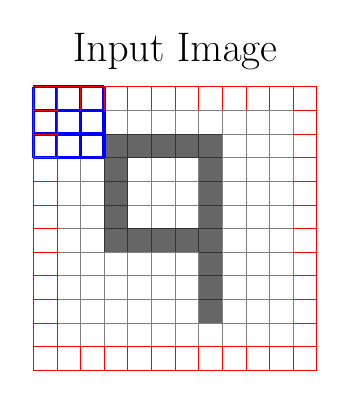
\begin{tikzpicture}[thick,scale=0.6, every node/.style={scale=0.6}]
  \node (text) at (2.5,6.25) {\Huge{Input Image}};
  % -=-=-=- ADDING ZEROS -=-=-=-
  \addNumbersConv
  % -=-=-=-=- REST OF IMAGE -=-=-=-=-
  \node (A) at (0,0) {};
  \node (B) at (5,5) {};

  \node (bA) at (3.5,4.5) {};
  \node (bB) at (3,0.5) {};

  \node (bC) at (1,4.5) {};
  \node (bD) at (3,4) {};

  \node (bE) at (1,4) {};
  \node (bF) at (1.5,2.5) {};

  \node (bG) at (1,2.5) {};
  \node (bH) at (3,2) {};

  \draw[step=0.5cm,gray,very thin] (A) grid (B);
  
  \fill[black,opacity=0.6] (bA) rectangle (bB) {};
  \fill[black,opacity=0.6] (bC) rectangle (bD) {};
  \fill[black,opacity=0.6] (bE) rectangle (bF) {};
  \fill[black,opacity=0.6] (bG) rectangle (bH) {};

  % -=-=-=-=- CONVOLUTION IMAGE PORTION -=-=-=-=-=-
  \node (cA) at (-0.5,4) {};
  \node (cB) at (1,5.5) {};

  \draw[step=0.5cm,blue,very thick,xshift=0cm,yshift=4cm] (cA) grid (cB);


  % -=-=-=-=- ZERO PADDING -=-=-=-=-
  \node (dA) at (-0.5,5) {};
  \node (dB) at (5.5,5.5) {};
  \node (dC) at (5,-0.5) {};
  \node (dD) at (5.5,5.5) {};
  \draw[step=0.5cm,red, very thin,xshift=0cm,yshift=0cm] (-0.5,-0.5) grid (5,0);
  \draw[step=0.5cm,red, very thin,xshift=0cm,yshift=0cm] (-0.5,0) grid (0,5);
  \draw[step=0.5cm,red, very thin,xshift=4cm,yshift=0cm] (dC) grid (dD);
  \draw[step=0.5cm,red, very thin,xshift=0cm,yshift=3cm] (dA) grid (dB);
\end{tikzpicture}\hspace{1cm}
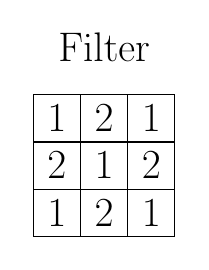
\begin{tikzpicture}[thick,scale=0.6, every node/.style={scale=0.6}]
  % -=-=-=-=- RESULTING IMAGE -=-=-=-=-
  \node (title) at (1.5,4) {\Huge{Filter}};
  \node (A) at (0,0) {};
  \node (B) at (3,3) {};
  \draw[step=1cm,black,thin] (A) grid (B);
  \node (a) at (0.5,0.5) {\Huge{$1$}};
  \node (b) at (1.5,0.5) {\Huge{$2$}};
  \node (c) at (2.5,0.5) {\Huge{$1$}};
  \node (d) at (0.5,1.5) {\Huge{$2$}};
  \node (e) at (1.5,1.5) {\Huge{$1$}};
  \node (f) at (2.5,1.5) {\Huge{$2$}};
  \node (g) at (0.5,2.5) {\Huge{$1$}};
  \node (h) at (1.5,2.5) {\Huge{$2$}};
  \node (i) at (2.5,2.5) {\Huge{$1$}};
\end{tikzpicture}\hspace{1cm}
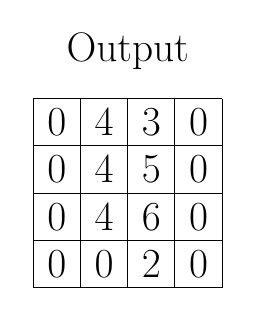
\begin{tikzpicture}[thick,scale=0.6, every node/.style={scale=0.6}]
  % -=-=-=-=- RESULTING IMAGE -=-=-=-=-
  \node(text) at (2,5) {\Huge{Output}};
  \node (A) at (0,0) {};
  \node (B) at (4,4) {};
  \draw[step=1cm,black,thin] (A) grid (B);
  \node (a) at (0.5,0.5) {\Huge{$0$}};
  \node (b) at (1.5,0.5) {\Huge{$0$}};
  \node (c) at (2.5,0.5) {\Huge{$2$}};
  \node (d) at (3.5,0.5) {\Huge{$0$}};

  \node (e) at (0.5,1.5) {\Huge{$0$}};
  \node (f) at (1.5,1.5) {\Huge{$4$}};
  \node (g) at (2.5,1.5) {\Huge{$6$}};
  \node (h) at (3.5,1.5) {\Huge{$0$}};

  \node (i) at (0.5,2.5) {\Huge{$0$}};
  \node (j) at (1.5,2.5) {\Huge{$4$}};
  \node (k) at (2.5,2.5) {\Huge{$5$}};
  \node (l) at (3.5,2.5) {\Huge{$0$}};

  \node (m) at (0.5,3.5) {\Huge{$0$}};
  \node (n) at (1.5,3.5) {\Huge{$4$}};
  \node (o) at (2.5,3.5) {\Huge{$3$}};
  \node (p) at (3.5,3.5) {\Huge{$0$}};
\end{tikzpicture}
\end{document}